\item Consider the LTI SISO system in Problem 2 of homework 5:
  \begin{equation}
    A =
    \begin{bmatrix}
      -2 & -2 & 0 \\
      0 & 0 & 1 \\
      0 & -3 & -4 
    \end{bmatrix}
    B =
    \begin{bmatrix}
      1 & 0 \\
      0 & 0 \\
      0 & 1
    \end{bmatrix}
    C =
    \begin{bmatrix}
      1 & 0 & 1 \\
      0 & 1 & 0
    \end{bmatrix}
  \end{equation}
  Recall that, in that homework, you designed a state feedback control law $\bar u(t) = -K\bar x(t)$ such that
  the eigenvalues of the closed-loop system because $\lambda_{d_1} = \lambda_{d_2} = -3$ and $\lambda_{d_3} = -4$.
  ie you have already obtained the control gain matrix $K$
  \begin{enumerate}
  \item Design a full-order observer with observer poles $\mu_{d_1} = -6, \mu_{d_2} = -7, \mu_{d_3}=-8$ using
    either methodd 1 in slide 121 or method 2 on slide 122 and verify the eigenvalues of
    $(A-LC)$. \\
    The first goal will be to reduce the multi-output model to a single
output model
\begin{equation}
v = \left[\begin{matrix}1.647 & 1.299\end{matrix}\right]
\end{equation}
the desired eigenvalues for the observer are: 
\begin{equation}
\lambda = -6, -7, -8
\end{equation}
Desired Characteristic equation
\begin{equation}
\Delta_d(\lambda) = \lambda^{3} + 21 \lambda^{2} + 146 \lambda + 336
\end{equation}
Desired Characteristic equation
\begin{equation}
\bar \alpha = \left[\begin{matrix}336\\146\\21\end{matrix}\right]
\end{equation}
Desired Characteristic equation
\begin{equation}
\Delta_d(\lambda) = \operatorname{PurePoly}{\left( \lambda^{3} + 6 \lambda^{2} + 11 \lambda + 6, \lambda, domain=\mathbb{Z} \right)}
\end{equation}
Desired Characteristic equation
\begin{equation}
\alpha = \left[\begin{matrix}6\\11\\6\end{matrix}\right]
\end{equation}
$\bar l$
\begin{equation}
  \bar l = \bar \alpha - \alpha = 
\end{equation}
\begin{equation}
  \bar l = \left[\begin{matrix}336\\146\\21\end{matrix}\right] - \\\left[\begin{matrix}6\\11\\6\end{matrix}\right] = 
\end{equation}
\begin{equation}
  \bar l = \left[\begin{matrix}330\\135\\15\end{matrix}\right]
\end{equation}
Calculate P
\begin{equation}
 Q = P.T = 
  \begin{bmatrix}
    (A.T)^2C.T & (A.T)C.T & C.T\\
  \end{bmatrix}
  \begin{bmatrix}
    1 & 0 & 0 \\
    \alpha_1 & 1 & 0 \\
    \alpha_2 & \alpha_1 & 1 \\
  \end{bmatrix}
\end{equation}\begin{equation}
  Q = \left[\begin{matrix}6.587 & -3.294 & 1.647\\22.453 & -8.234 & 1.299\\12.921 & -5.289 & 1.647\end{matrix}\right]\left[\begin{matrix}1 & 0 & 0\\6 & 1 & 0\\11 & 6 & 1\end{matrix}\right]
\end{equation}
\begin{equation}
  Q = \left[\begin{matrix}4.94 & 6.587 & 1.647\\-12.667 & -0.443 & 1.299\\-0.697 & 4.592 & 1.647\end{matrix}\right]
\end{equation}
\begin{equation}
  P = Q.T = \left[\begin{matrix}4.94 & -12.667 & -0.697\\6.587 & -0.443 & 4.592\\1.647 & 1.299 & 1.647\end{matrix}\right]
\end{equation}
\begin{equation}
  l = P^{-1} \bar l  = \left[\begin{matrix}-187.492\\-114.975\\287.261\end{matrix}\right]
\end{equation}
\begin{equation}
  L = lv  = \left[\begin{matrix}-308.762 & -243.466\\-189.34 & -149.299\\473.061 & 373.02\end{matrix}\right]
\end{equation}
To verify the equations use: eig($ A - LC$)
\begin{equation}
  \vert \lambda - (A - LC) \vert  = \operatorname{PurePoly}{\left( 1.0 \lambda^{3} + 21.0 \lambda^{2} + 146.0 \lambda + 336.0, \lambda, domain=\mathbb{R} \right)}
\end{equation}
\begin{enumerate}
\item $\lambda = -6.0$
\item $\lambda = -7.0$
\item $\lambda = -8.0$
\end{enumerate}

  \item We know that using seperation principle we can design an observer-basesd feedback control. In eqs 69, 70
    of the slides, let the control input be $\bar u(t) = -K\hat x(t)$ with the control gain matrix $k$ obtained
    obtained in either part a or part b of problem 2 of homework 5, and let the observer gain matrix $L$ be that
    obtained in part (a) above. Simulate and plot the state response of the closed-loop system assuming that the
    initial conditions of the states and estimated state are
    $\bar x_0 = \begin{bmatrix} 1 \\ -1 \\ 2.3 \end{bmatrix}$ and 
    $\hat x_0 = \begin{bmatrix} 1.7 \\ -0.3 \\ 2.5 \end{bmatrix}$ respectively. In your plots ensure that
    the transient response and system convergence are depicted clearly.
    \begin{figure}[H]
  \begin{center}
    \makebox[\textwidth]{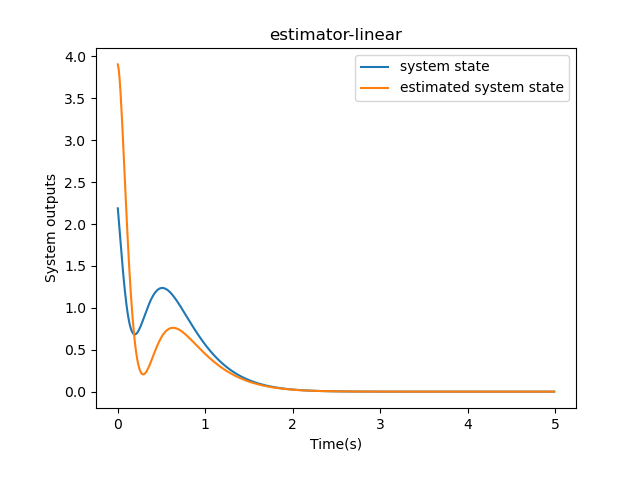
\includegraphics[max width=\textwidth]{../resources/estimator-linear.png}}
  \end{center}
  \caption{Estimator in NonLinear performance}
  \label{fig:estimator-linear}
\end{figure}

  \item Design a reduce order observer with observer pole $\mu_{d_1} = -8$. No need for computer simulation\\
    \begin{equation}
      F = -8
    \end{equation}
    \begin{equation}
      G = 1
    \end{equation}
    \begin{equation}
      TA - FT = GC =
      T
      \begin{bmatrix}
        -2 & -2 & 0 \\
        0 & 0 & 1 \\
        0 & -3 & -4 
      \end{bmatrix}
      - 8T = 
      \begin{bmatrix}
        1 & 0 & 1 \\
        0 & 1 & 0
      \end{bmatrix}
    \end{equation}
    some very manual brute forcing later
    \begin{equation}
      T =
      \begin{bmatrix}
        0.1667 & -0.5 & -0.14583333 \\
        0 & 0.1143 & -0.0285
      \end{bmatrix}
    \end{equation}
  \end{enumerate}
  